\subsection{Privilege Level Switching}
\label{sec:faults}

Applications software needs a method to invoke the kernel, because it cannot
perform privileged operations, such as network or disk I/O. At the same time,
ring 3 software cannot be offered the ability to jump arbitrarily into kernel
code, because that would compromise the kernel's ability to isolate
applications and enforce security invariants.
\footnote{For example, when an application wishes to write a file to the disk,
the kernel must check if the application's user has access to that file. If the
ring 3 code could perform an arbitrary jump in kernel space, it would be able
to skip the access check.}
Therefore, the processor has designated methods for switching privilege levels,
which protect the integrity of the privileged software.  This section describes
the privilege switching mechanisms that impact the SGX design. Furthermore,
the process of calling code inside an enclave is similar to switching
privilege levels, because the enclave code must be protected from

% Performing Fast Calls to System Procedures with the SYSENTER and SYSEXIT
%     Instructions: SDM S 5.8.7
% Architectural MSRs: SDM S 35.1

\begin{figure}[hbt]
  \center{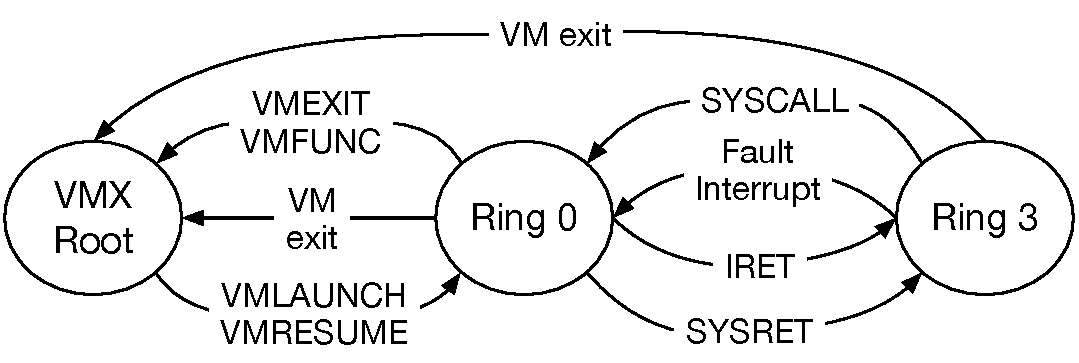
\includegraphics[width=85mm]{figures/cpu_ring_switch.pdf}}
  \caption{
    Modern privilege switching methods in the 64-bit Intel architecture.
  }
  \label{fig:cpu_ring_switch}
\end{figure}

On modern processors, application software uses the SYSCALL instruction to
to invoke ring 0 code, and the kernel uses SYSRET to switch the privilege level
back to ring 3. SYSCALL jumps into a predefined kernel location, which is
specified by writing to \textit{architectural Model Specific Registers (MSRs)}.
\footnote{Despite the ``model-specific'' in MSR, \textit{architectural} MSRs
are a part of the Intel architecture, and their semantics are stable across
processor generations.} MSRs can only be read or written by ring 0 code,
therefore application softeware cannot execute arbitrary kernel code.

% Interrupt and Exception Handling: SDM S 6.1, S 6.2

The processor also performs a switch from ring 3 to ring 0 when a hardware
exception (also called \textit{fault}) occurs in application software.  Some
exceptions indicate bugs in the application software, whereas other exceptions
require kernel action. A \textit{general protection fault} (\#GP) occurs when
software attempts to perform a disallowed action, such as setting the CR3
register from ring 3. A \textit{page fault} (\#PF) occurs when address
translation encounters a page table entry whose P flag is 0, or attempting to
use a page in a way inconsistent with the access bits in its page table entry,
for example accessing a page whose S bit is set from ring 3.

When an exception occurs, the CPU performs a ring switch, and calls the
\textit{fault handler} for that exception. The locations of the fault handlers
in the kernel code is specified in the first 32 entries of the Interrupt
Descriptor Table (IDT), whose structure is shown in Table~\ref{fig:idt_entry}.
The IDT's physical address is stored in the IDTR register, which can only be
accessed by ring 0 code. Kernels protect the IDT memory using page tables, so
that ring 3 software cannot access it.

\begin{table}[hbt]
  \center{\begin{tabular}{| l | l |}
  \hline
  \textbf{Bits} & \textbf{Field}\\
  \hline
  111..48 & Handler RIP 63..16 \\
  \hline
  47 & Present (P) \\
  \hline
  46..45 & Zero for ring 0 \\
  \hline
  43..40 & Type (14 or 15 in 64-bit mode) \\
  \hline
  34..32 & Interrupt Stack Table \\
  \hline
  31..16 & Handler CS \\
  \hline
  15..0 & Handler RIP 15..0 \\
  \hline
  \end{tabular}}
  \caption{
    The fields of an IDT entry in 64-bit mode. Each entry points to a fault or
    interrupt handler.
  }
  \label{fig:idt_entry}
\end{table}




page fault (\#PF), and the OS kernel is responsible for loading the page back
into RAM and resuming execution. If an EPT entry has the P flag set to 0, the
CPU performs a VM exit, and the hypervisor has an opportunity to bring the page
into RAM.

i

Faults can occur when
Page Fault

Figure~\ref{fig:cpu_ring_switch} shows




